\documentclass[12pt,a4paper]{article}
\usepackage[warn]{mathtext}
\usepackage[utf8]{inputenc}
\usepackage[english,russian]{babel}
\usepackage{amsmath}
\usepackage{amssymb}
\usepackage{latexsym}
\usepackage{svg}
\usepackage{pgfplots}
\pgfplotsset{compat=1.9}

\usepackage{listings}

\usepackage{color}

\definecolor{dkgreen}{rgb}{0,0.6,0}
\definecolor{gray}{rgb}{0.5,0.5,0.5}
\definecolor{mauve}{rgb}{0.58,0,0.82}

\lstset{ %
	language=python,                % Язык программирования 
	numbers=left,                   % С какой стороны нумеровать
	stepnumber=1,                   % Шаг между линиями. Если 1, то будет пронумерована каждая строка
	frame=single,	
}
\usepackage[left=30mm,right=10mm,
top=20mm,bottom=20mm,bindingoffset=0cm, nohead, footskip=10mm]{geometry}

\usepackage{sverb}
\usepackage{graphicx}
\usepackage{pdfpages}
\usepackage[absolute,overlay]{textpos}

\begin{document}
	\begin{titlepage}
		\begin{textblock*}{13cm}(0cm,0cm)
			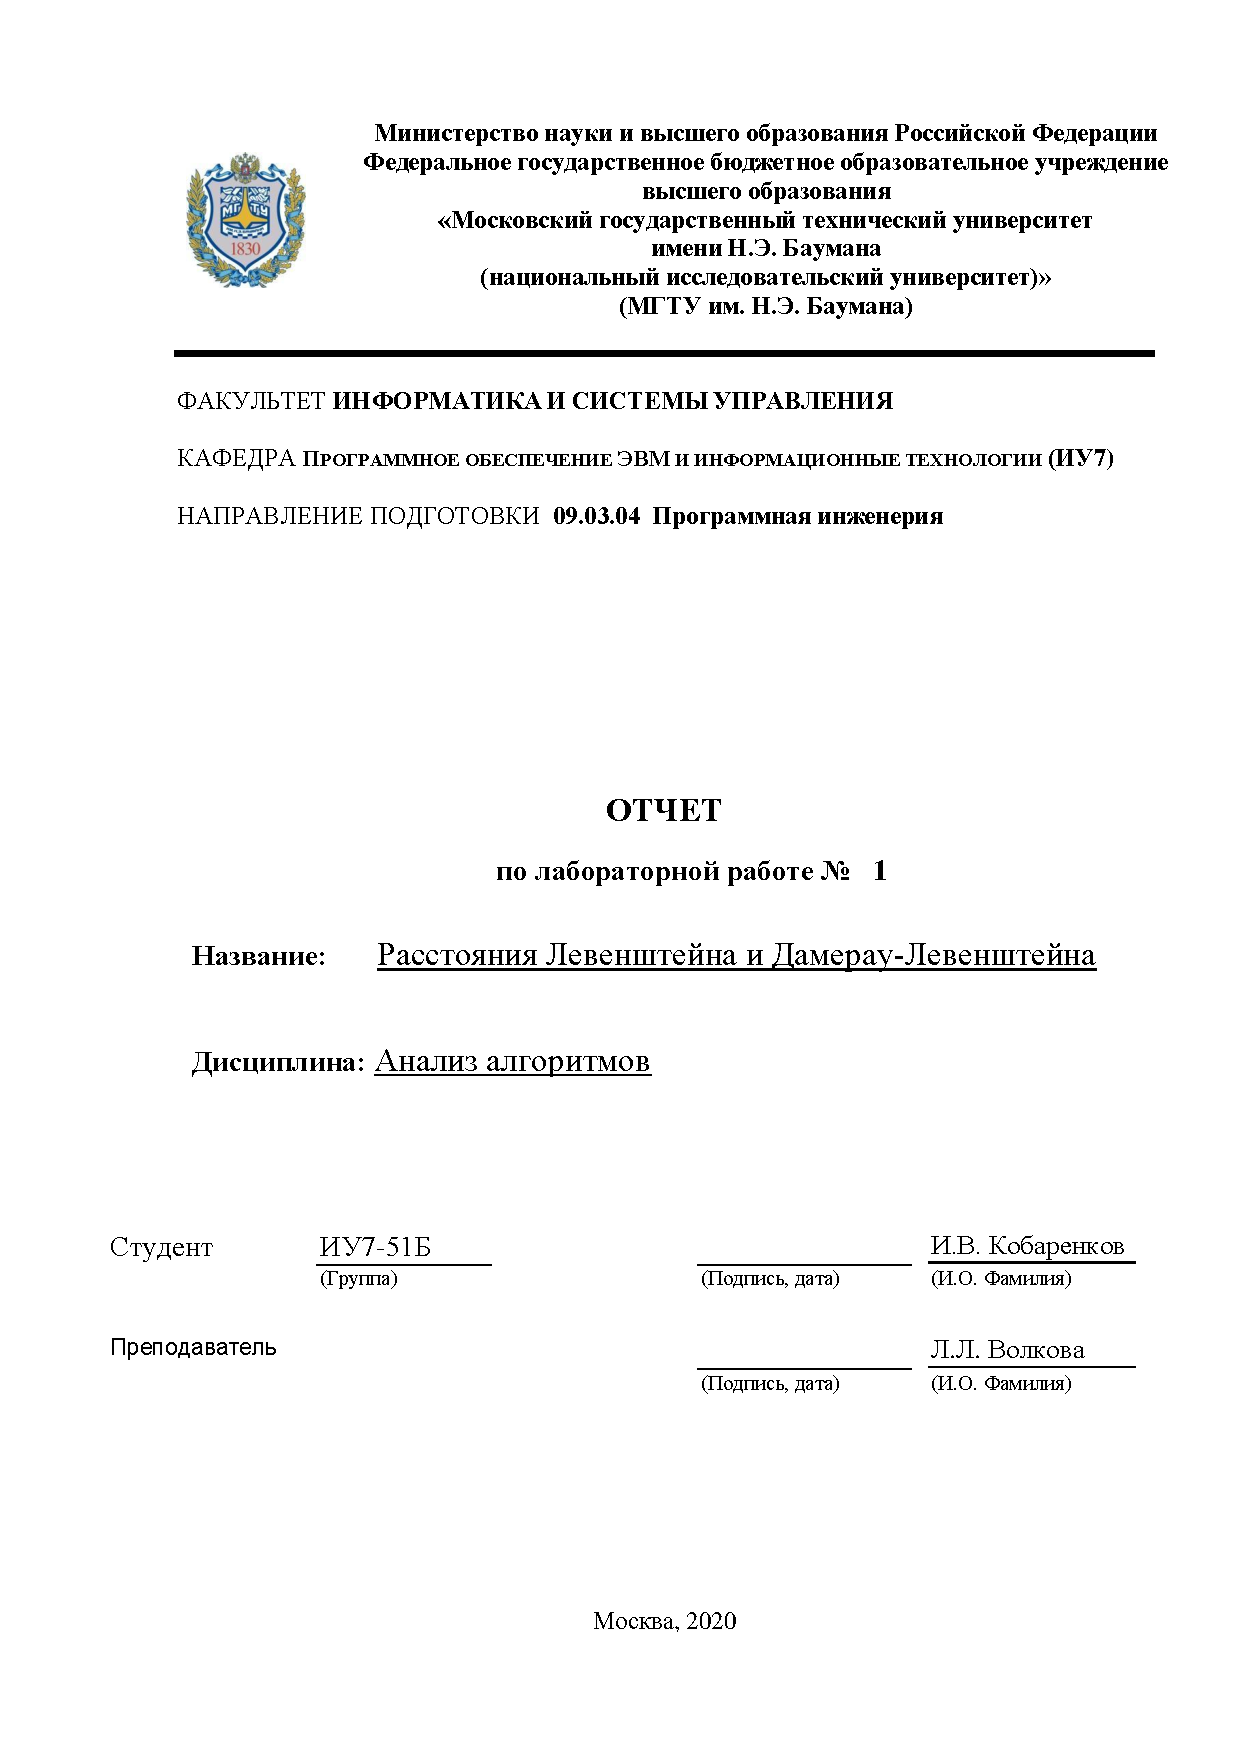
\includegraphics{title_01}
		\end{textblock*}
	\end{titlepage}
\hspace{0pt}
\clearpage

\tableofcontents
\clearpage

\addcontentsline{toc}{section}{Введение}
%//////////////////////////////////////////////////////////////////
\section*{\Huge Введение}
Расстояние Левенштейна (редакционное расстояние) - это минимальное кол-во редакторских операций, которое необходимо для превращения одной строки в другую.\\
\\
Применение.\\
1) Поисковики (Google), автоисправления\\
2) Биоинформатика\\
\\
Задания для данной ЛР:\\
1) изучение алгоритмов Левенштейна и Дамерау-Левенштейна нахождения расстояния между строками;\\
2) получение практических навыков реализации указанных алгоритмов: двух алгоритмов в матричной версии и одного из алгоритмов в рекурсивной версии;\\
3) сравнительный анализ линейной и рекурсивной реализаций выбранного алгоритма определения расстояния между строками по затрачиваемым ресурсам (времени и памяти);\\
4) эксперементальное подтверждение различий во временной эффективности рекурсивной и нерекурсивной реализаций выбранного алгоритма определения расстояния между строками при помощи разработанного программного обеспечения на материале замеров процессорного времени выполнения реализации на варьирущихся длинах строк;\\
5) описание и обоснование полученных результатов в отчете о выполненной лабораторной работе.\\
\clearpage

\section{Аналитическая часть}
Задача по нахождению расстояния Левенштайна заключается в поиске минимального количества операций:\\
\textbf{Вставка (I - Insert)}\\
\textbf{Удаление (D - Delete)}\\
\textbf{Замена (R - Replace)}\\
\textbf{Совпадение (M - Match)}\\
Для превращения одной строки в другую.\\
В алгоритме Далмерау-Левенштайна добавляется ещё одна операция:\\
\textbf{Транспозиция(T)}\\
Все операции, кроме "Совпадения" имею штраф 1. Операция "Совпадения" имеет штраф 0.
\newpage
\subsection{Описание алгоритмов}

\subsubsection{Рекурсивный алгоритм Левенштейна}
Введём понятие D(s1, s2) = минимальному количеству редакторских операций, с помощью которых строка s1 преобразуется в строку s2.
Тогда рекурсивный алгоритм Левенштейна можно записать следующим образом:\\
$
D(i, j) = \begin{cases}
	0, i = 0, j = 0 \\
	i, j = 0, i > 0 \\
	j, i = 0, j > 0 \\
	min(D(S_{1}[1, ..., i], S_{2}[1, ..., j - 1]) + 1,\\
	D(S_{1}[1, ..., i - 1], S_{2}[1, ..., j]) + 1,\\
	D(S_{1}[1, ..., i - 1], S_{2}[1, ..., j - 1]) + \\
	\left[
	\begin{gathered}
	0, if S_{1}[i] = S_{2}[j],\\
	1, else
	\end{gathered}
	\right.
\end{cases}
$

\subsubsection{Матричный алгоритм Левенштейна}
Вводится матрица, размерностью $[Len(S_{1}) + 1 \textbf{X} Len(S_{2}) + 1]$\\
Первая строки и столбец матрицы заполняются от 0 до Len(S) (первые 3 пункта системы из предыдущего пункта).\\
\\
\begin{equation*}
A = \left(
\begin{array}{ccccccc}
 & \emptyset & \text{С} & \text{Т} & \text{О} & \text{Л} & \text{Б}\\
\emptyset & 0 & 1 & 2 & 3 & 4 & 5\\
\text{Т} & 1 & & & & & \\ 
\text{Е} & 2 & & & & & \\
\text{Л} & 3 & & & & & \\
\text{О} & 4 & & & & & \\
\end{array}
\right)
\end{equation*}

Далее для нахождения ответа применяется последняя формула из системы, описанной в предыдущем пункте.

\begin{equation*}
A = \left(
\begin{array}{ccccccc}
& \emptyset & \text{С} & \text{Т} & \text{О} & \text{Л} & \text{Б}\\
\emptyset & 0 & 1 & 2 & 3 & 4 & 5\\
\text{Т} & 1 & 1 & 1 & 2 & 3 & 4 \\ 
\text{Е} & 2 & 2 & 2 & 2 & 3 & 4 \\
\text{Л} & 3 & 3 & 3 & 3 & 2 & 3 \\
\text{О} & 4 & 4 & 4 & 3 & 3 & \textbf{3} \\
\end{array}
\right)
\end{equation*}
\\
Ответ в правом нижнем углу.\\
\\
Чтобы определить, какая именно цепочка преобразований привела к ответу представим матрицу как карту высот: нужно спуститься на санках из клетки с ответом в левый верхний угол. В нашем случае:\\
$\textbf{I}$: ТЕЛО $\rightarrow$ СТЕЛО\\
$\textbf{M}$: Т = Т\\
$\textbf{R}$: Е $\rightarrow$ О\\
$\textbf{M}$: Л = Л\\
$\textbf{R}$: О $\rightarrow$ Б\\


\subsubsection{Рекурсивно-матричный алгоритм Левенштейна}
Аналогичен алогритму из предыдущего пункта с той лишь разницей, что матрица начинает заполнение "с конца". Вычисляем значение ячейки матрицы только в том случае, если значения там ещё нет (аналогично $\infty$ в алгоритме Дейкстры). Ответ всё так же в правом нижнем углу.

\section{Конструкторская часть}
\textbf{Требования к вводу:}\\
1) на вход подаются две строки;\\
2) одна и та же буква в разном регистре считается как разный символ.\\
\textbf{Требования к программе:}:\\
1) Две пустые строки являются корректным вводом, который программа должна обработать.
\clearpage
\subsection{Разработка алгоритмов} % Сюда схемы алгоритмов
В данном разделе представлены схемы реализуемых алгоритмов.
\subsubsection{Схема рекурсивной реализации алгоритма Левенштейна}
\begin{center}	
	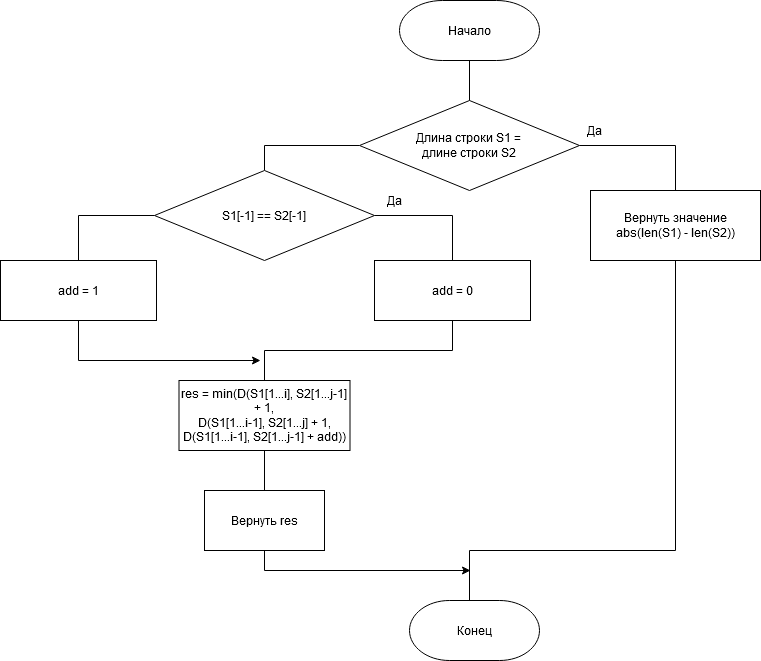
\includegraphics[width=0.9\linewidth]{lev_rec}\\
	Рис. 1: Cхема рекурсивного алгоритма Левенштейна
\end{center}
\clearpage
\subsubsection{Схема матричной реализации алгоритма Левенштейна}
\begin{center}	
	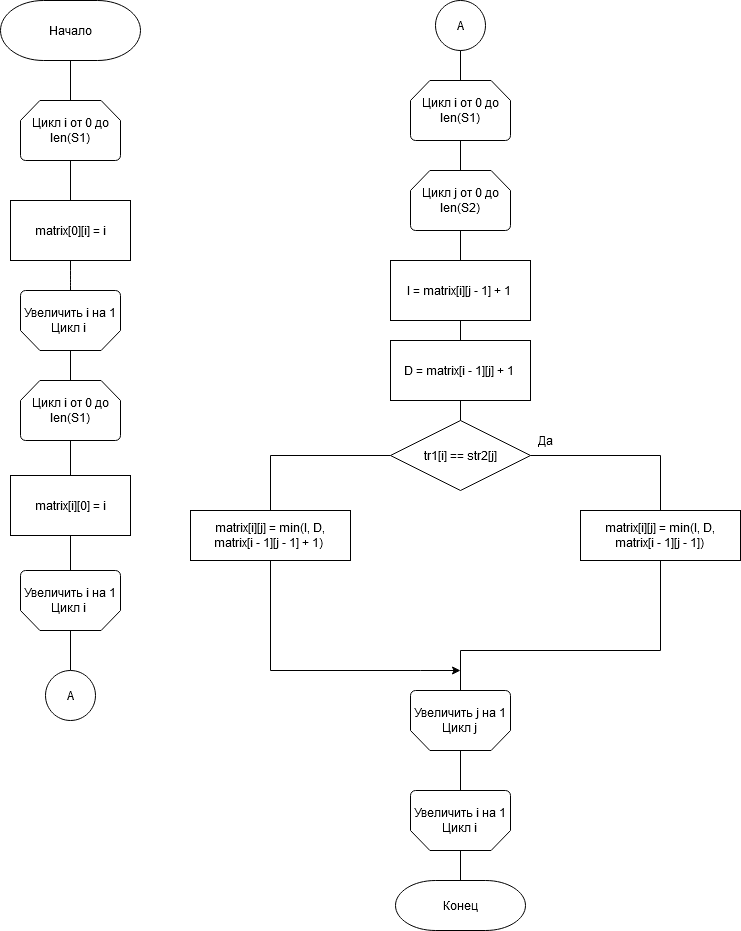
\includegraphics[width=.9\linewidth]{lev_matr}\\
	Рис. 2: Cхема матричной реализации алгоритма Левенштейна
\end{center}
\clearpage
\subsubsection{Схема рекурсивного матричного алгоритма Левенштейна}
\begin{center}
	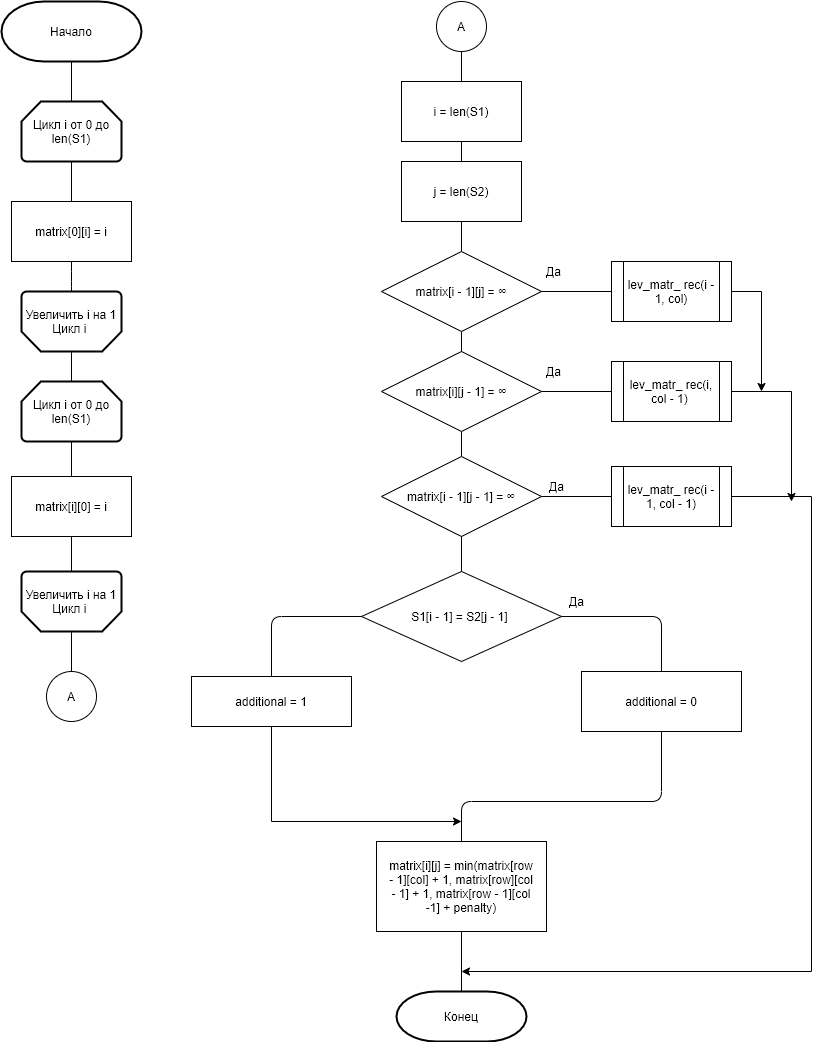
\includegraphics[width=1\linewidth]{lev_matr_rec}\\
	Рис. 3: Cхема рекурсивной матричной реализации алгоритма Левенштейна
\end{center}
\clearpage
\subsubsection{Схема алгоритма Дамерау-Левенштейна}
\begin{center}
	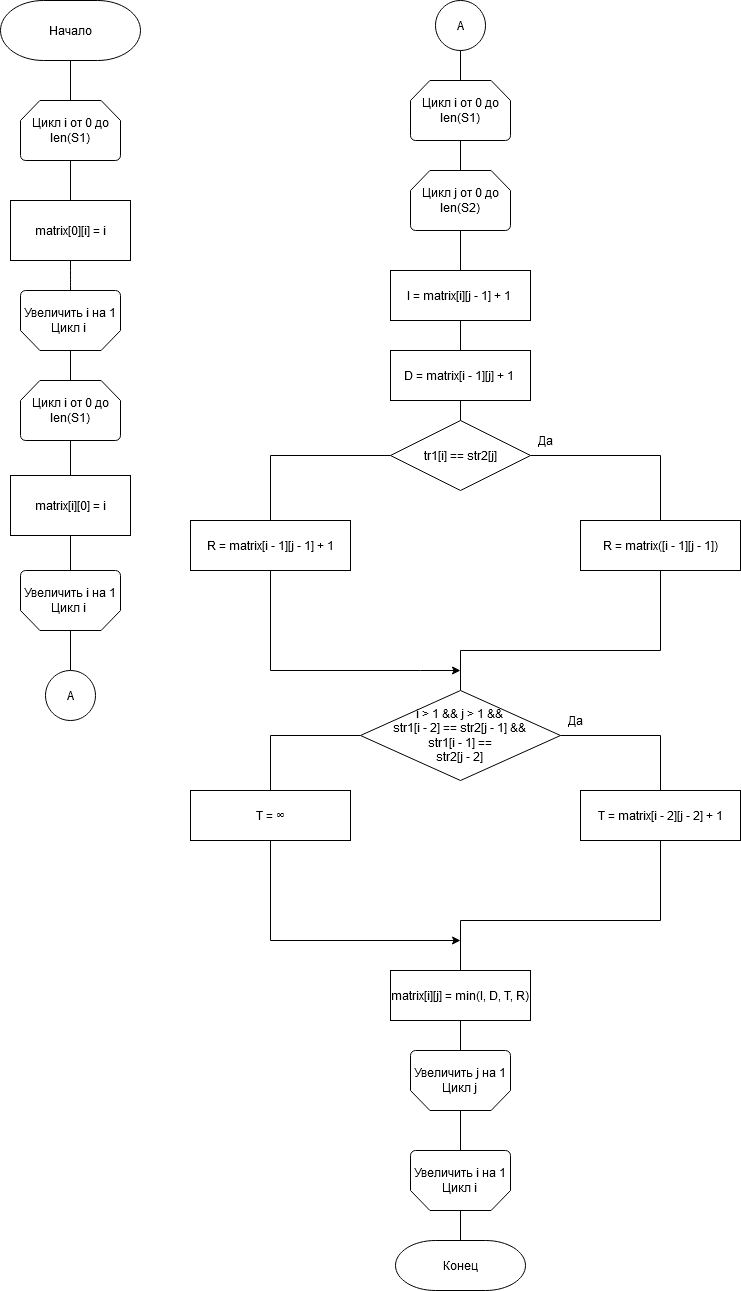
\includegraphics[width=.67\linewidth]{dam_lev}\\
	Рис. 4: Схема алгоритма Дамерау-Левенштейна
\end{center}
\clearpage

\section{Технологическая часть}
В данном разделе будет описана технологическая часть лабораторной работы: требования к ПО, листинг кода, сравнительный анализ всех алгоритмов.
\subsection{Требования к программному обеспечению}
Входные данные: два слова: str1, str2\\
Выходные данные: редакционное расстояние данных слов, а также матрица решения для матричных реализаций\\
Среда выполнения: Windows 10 x64
\subsection{Средства реализации}
Для выполнения данной лабораторной работы использовался ЯП Python 3.9.0 \\
\subsection{Листинг кода}
В данном разделе будет представлен листинг кода разработанных алгоритмов.\\

\subsubsection{Рекурсивный алгоритм Левенштейна}
\begin{flushleft}
	Листинг 1: Рекурсивный алгоритм Левенштейна
	\lstinputlisting[language=python]{lev_rec.py}
\end{flushleft}
\clearpage

\subsubsection{Матричный алгоритм Левенштейна}
\begin{flushleft}
	Листинг 2: Матричный алгоритм Левенштейна
	\lstinputlisting[language=python]{lev_matr.py}
\end{flushleft}

\subsubsection{Рекурсивный матричный алгоритм Левенштейна}
\begin{flushleft}
	Листинг 3: Рекурсивный матричный алгоритм Левенштейна
	\lstinputlisting[language=python]{lev_matr_rec.py}
\end{flushleft}
\clearpage

\subsubsection{Алгоритм Дамерау-Левенштейна}
\begin{flushleft}
	Листинг 4: Алгоритм Дамерау-Левенштейна
	\lstinputlisting[language=python]{dam_lev.py}
\end{flushleft}
\clearpage

\subsection{Сравнительный анализ матричной и рекурсивной реализаций}
Рекурсивная версия алгоритма работает существенно медленне матричной реализации ввиду многократного вызова функции. На каждый вызов необходимо производить соответствующие операции со стеком. Для уменьшения затрат по времени (на копирование) и на дополнитульную память строки можно \textbf{передавать по ссылке} Тогда на каждую строку, независимо от её размера будет выделяться фиксированное число байт (количество зависит от разрядности системы). Однако даже такие ухищрения не способны избавить от главного недостатка - повторного вычисления тех значений, которые были посчитаны на более ранних этапах рекурсии.
В матричных реализация будет затрачена дополнительная память на хранение матриц и дополнительных переменных в цикле, однако скорость работы подобной реализации будет значительно быстрее рекурсивной.
\subsubsection{Теоретический анализ затрачиваемой памяти}
\textbf{Рекурсивная реализация алгоритма Левенштейна}. Для получения конечной оценки затрачиваемой памяти необходимо память, затрачиваемую на единичный вызов функции умножить на максимальную глубину рекурсии, то есть на n + m, где n и m - длины сравниваемых строк s1 и s2 соответственно.
\begin{enumerate}
	\item ссылки на строки s1, s2: (m + n) * sizeof(reference),
	\item длины строк: 2 * sizeof(int),
	\item дополнительная переменная внутри алгоритма: sizeof(int)
	\item адрес возврата
\end{enumerate}

\textbf{Матричная реализация алгоритма Левенштейна}
\begin{enumerate}
	\item строки: sizeof(str) * (n + m)
	\item матрица: sizeof(int) * (n + 1) * (m + 1)
	\item дополнительная переменная внутри алгоритма: sizeof(int)
\end{enumerate}

\textbf{Рекурсивный матричный алгоритм Левенштейна}. Аналогично обычному рекурсивному алгоритму для получения конечной оценки затрачиваемой памяти необходимо память, затрачиваемую на каждом рекурсивном вызове умножить на максимальную глубину рекурсии.
\begin{enumerate}
	\item строки: sizeof(str) * (n + m)
	\item матрица: sizeof(int) * (n + 1) * (m + 1)
\end{enumerate}
При каждой необходимости предварительного подсчёта значения (рек. вызова)
\begin{enumerate}
	\item передача строки и столбца: 2 * sizeof(int)
	\item дополнительная переменная: sizeof(int)
	\item адрес возврата
\end{enumerate}

\textbf{Матричная реализация алгоритма Дамера-Левенштейна}
\begin{enumerate}
	\item строки: sizeof(str) * (n + m)
	\item матрица: sizeof(int) * (n + 1) * (m + 1)
	\item дополнительная переменная внутри алгоритма: sizeof(int)
\end{enumerate}

\subsection{Описание тестирования} % описать, какие тесты будут проведены ВСЕ ТЕСТЫ ПРОЙДЕНЫ УСПЕШНО
\subsubsection{Интерфейс программы}
При запуске программы пользователя встречает меню выбора реализаций алгоритма:\\
\begin{center}
	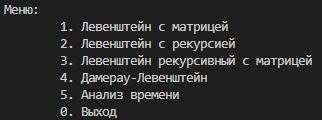
\includegraphics{menu}\\
	Рис.5: Меню программы
\end{center}
После выбора необходимой реализации пользователю предлагают ввести строки s1 и s2. После ввода программа выдаёт результат:\\
\begin{center}
	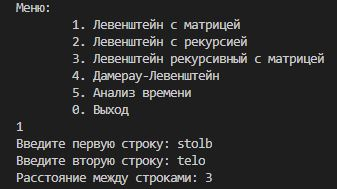
\includegraphics{examp}\\
	Рис.6: Ввод строк и результат работы программы
\end{center}
\subsubsection{Тесты}
Тестирование было организовано с помощью библиотеки  \textbf{unittest}.
Было создано две вариации тестов:

В первой сравнивались результаты функции с реальным результатом.

Во второй сравнивались результаты двух функций(рекурсивной и табличной).
При сравнении результатов двух функций использовалась функция random string, которая генерирует случайную строку нужной длины.
\begin{center}
	Листинг 5: Функция random string
	\lstinputlisting[language=C++]{random_string.py}
\end{center}
\clearpage

\section{Исследовательская часть}
%В данной части работы будут приведены примеры работы программ, а также анализ алгоритмов на основе эксперементальных данных.
\subsection{Примеры работы}
Проверка на пустые строки:
\begin{lstlisting}
	source = ""
	target = ""
	Recursive Levenshtein: 0
	Table Levenshtein: 0
	Recursive-Table Levenshtein: 0
	Table Damerau-Levenshtein: 0
\end{lstlisting}
Проверка на на равенство строк:
\begin{lstlisting}
	source = "abc"
	target = "abc"
	Recursive Levenshtein: 0
	Table Levenshtein: 0
	Recursive-Table Levenshtein: 0
	Table Damerau-Levenshtein: 0
\end{lstlisting}

Операция удаления:
\begin{lstlisting}
	source = "abc"
	target = "ab"
	Recursive Levenshtein: 1
	Table Levenshtein: 1
	Recursive-Table Levenshtein: 1
	Table Damerau-Levenshtein: 1
\end{lstlisting}

Операция замены:
\begin{lstlisting}
	source = "abf"
	target = "abc"
	Recursive Levenshtein: 1
	Table Levenshtein: 1
	Recursive-Table Levenshtein: 1
	Table Damerau-Levenshtein: 1
\end{lstlisting}

Операция вставки:
\begin{lstlisting}
	source = "ab"
	targer = "abc"
	Recursive Levenshtein: 1
	Table Levenshtein: 1
	Recursive-Table Levenshtein: 1
	Table Damerau-Levenshtein: 1
\end{lstlisting}
\clearpage
Операция перестановки:
\begin{lstlisting}
	source = "abc"
	target = "acb"
	Recursive Levenshtein: 2
	Table Levenshtein: 2
	Recursive-Table Levenshtein: 2
	Table Damerau-Levenshtein: 1
\end{lstlisting}
\subsection{Постановка эксперимента по замеру времени}
Для замера времени было использовано средство \textbf{QueryPerformanceCounter}\\
Были произведены замеры для строк длиной от 0 до 1000.\\
Для каждой размерности было проведено 100 вызовов функции. После чего получившеесся время было поделено на 100. Таким образом было получено аппроксимированное значение времени выполнения функции\\
Результаты замеров процессорного времени:\\
\begin{center}
	Был проведен замер времени работы каждого из алгоритмов.
\end{center}

\begin{center}
	\begin{tabular}{|c c c c c|} 
 	\hline
	Длина строки & Lev(R) & Lev(MR) & Lev(M) & DamLev(M) \\ [0.5ex] 
 	\hline\hline
	3 & 506 & 500.7 & 180.3 & 170.1\\
 	\hline
	5 & 2027.3 & 1820.2 & 200.3 & 223.3\\
 	\hline
 	7 & 28388.8 & 24681.7 & 292.3 & 285.1\\
 	\hline
 	9 & 645759  & 538134 & 311.7 & 294.5\\
 	\hline
	11 & 12511100 & 11792800 & 331 & 391.6\\
	\hline
	\end{tabular}
\end{center}

\begin{center}
	\begin{tikzpicture}
	\begin{axis}
	\addplot coordinates {
		(0, 0)(1, 0.000006) (2,  0.000014) (3,  0.000063) (4, 0.000442) (5,  0.00150) (6,  0.00611) (7,  0.04878) (8, 1.05122) (9, 1.20921) (10, 4.4408)
	};
	\addplot coordinates {
	(0, 0) (1,  0.00002) (2,  0.000016) (3,  0.00002) (4, 0.00002) (5,  0.00005) (6, 0.000039) (7,  0.00010) (8,  0.000079) (9, 0.0007245) (10, 0.0005613)
	};
	\addplot coordinates {
		(0, 0)(1,  0.00002) (2,   0.00009) (3,  0.000111 ) (4, 0.000224) (5,  0.000415) (6,  0.000766) (7,  0.001094 ) (8,  0.000865 ) (9, 0.000775) (10, 0.001896)
	};
	\addplot coordinates {
		(0, 0)(1,   0.000006) (2, 0.000009) (3, 0.00002) (4, 0.00003) (5,  0.00002) (6,  0.00003) (7, 0.00011) (8,  0.0007497 ) (9, 0.0009417
) (10, 0.0011017)
	};
	\end{axis}
	\end{tikzpicture}
	\\
	Легенда:\\
	Синий цвет - Рекурсивная реализация\\
	Коричныевый цвеи - Рекурсивная матричная реализация\\
	Чёрный цвет - Алгоритм Дамерау-Левенштейна\\
	Красный цвет - Обычная матричная реализцаия\\
	
\end{center}
\subsection{Сравнительный анализ на материале экспериментальных данных}
Теоретические расчёты подтвердились результатами, полученными на пратике: рекурсивный алгоритм ввиду многократного вызова функции и пересчёта уже известных значений выполняется крайне долго, рекурсивная матричная реализация выполняется быстрее, но всё равно из-за операций со стеком и вызовом самой себя уступает по времени обычной матричной реализации. Алгоритм Дамерау-Левенштейна уступает по времени обычной матричной реализации ввиду дополнительной проверки на перестановку символов.
\clearpage
\addcontentsline{toc}{section}{Заключение}
%//////////////////////////////////////////////////////////////////
\section*{\Huge Заключение}
В ходе работы были изучены алгоритмы нахождения расстояний Левенштейна и Дамерау–Левенштейна, применена методика динамического программирования для реализации указанных алгоритмов, а также произведён сравнительный анализ линейной и рекурсивной реализации алгоритмов. Было установлено, что обычный рекурсивный алгоритм занимает меньше памяти по сравнению с матричными реализациями, однако за быстродействие матричных алгоритмов приходится расплачиваться памятью.
\end{document}